We can visualize this in two dimensions in the following figure:

\begin{center}
    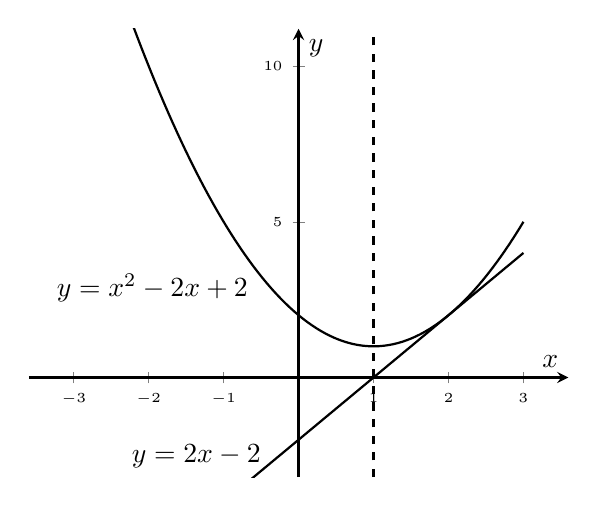
\begin{tikzpicture}[scale=1.0]
        \begin{axis}[
            axis lines=middle,
            xlabel=$x$,
            ylabel=$y$,
            xmin=-3, xmax=3,
            ymin=-2, ymax=10,
            % xtick={-2, -1, 0, 1, 2},
            % ytick={-2, 2, 4, 6, 8, 10},
            ticklabel style={font=\tiny},
            enlargelimits=true,
            thick]
            % Quadratic function
            \addplot[color=black, domain=-3:3, samples=101] {x^2 - 2*x + 2};
            \node[label={-45:{$y=x^2 - 2x + 2$}}] at (axis cs:-3.5,4) {};
            
            % Derivative function
            \addplot[color=black, domain=-3:3, samples=101] {2*x - 2};
            \node[label={-45:{$y=2x-2$}}] at (axis cs:-2.5,-1.5) {};

            \draw[dashed] (1,\pgfkeysvalueof{/pgfplots/ymin}) -- (1,\pgfkeysvalueof{/pgfplots/ymax});
        \end{axis}
    \end{tikzpicture}
\end{center}
